\documentclass{article} % Default font size and left-justified equations
% \documentclass{book}

\usepackage[
  margin=0.7in,
  % includefoot,
  % footskip=30pt,
]{geometry}

\usepackage{natbib}
\usepackage{enumitem}
\usepackage{amsmath,amsfonts}
\usepackage{graphicx}
\usepackage{framed}
\usepackage{subcaption}
\usepackage[T1]{fontenc}%
\usepackage[utf8]{inputenc}%
\usepackage{mathrsfs}%
\usepackage{amssymb}%
\usepackage{amsthm}%
\usepackage{graphicx}
\usepackage{hyperref}
\usepackage{environ}
\usepackage{framed}
\usepackage{mdframed} 
\usepackage{wrapfig} 
\usepackage{booktabs}
\usepackage{tabularx} 
\usepackage{array}
\usepackage[font=small]{caption} 
\usepackage{xspace}  
\usepackage[osf,sc]{mathpazo}
\usepackage{pbox}
\usepackage{listings}
\usepackage{tikz}
\usepackage{bm}
\usepackage[strict]{changepage}
\usepackage{mleftright}
\usepackage{appendix}%
\usepackage[all]{xy} 
\setcounter{tocdepth}{3}
\setcounter{secnumdepth}{3}
\usepackage[ruled,vlined]{algorithm2e}
\usepackage{framed}
\usepackage{wrapfig}
\usepackage{pythonhighlight}
\usepackage{tikz}
\usetikzlibrary{arrows}
\usetikzlibrary{arrows.meta}
\usetikzlibrary{shapes.geometric}
\usetikzlibrary{positioning, arrows, automata, calc}
\usepackage{transparent}
\usepackage[many]{tcolorbox}
\usepackage{tikz}
\usetikzlibrary{shapes.geometric}
\usetikzlibrary{positioning, arrows, automata, calc}

\newtcolorbox[]{your_solution}[1][]{
    % breakable,
    enhanced,
    nobeforeafter,
    colback=white,
    title=Your Answer,
    sidebyside align=top,
    box align=top,
    #1
}
\newcommand{\mybox}[1]{
\noindent
\fbox{\parbox{0.955\textwidth}{%
\noindent\texttt{#1}
}
}
}

\newcommand{\filler}{ . . . . . }
\newcommand{\choice}{\hspace{0.5cm}$\square$}
\newcommand{\identity}{\mathbf{I}} 
\newcommand{\paran}[1]{\left( #1 \right)}

%% PLEASE USE THESE MACROS WHEN WRITING THE SOLUTIONS 
\newcommand{\solution}[1]{\textcolor{blue}{Answer: \em #1}
} % show
%\newcommand{\solution}[2]{#2} % hide

\newcommand{\extracredit}{{\color{purple}\textbf{Extra Credit:}}}

\newcommand{\additionalNotes}{
\noindent\textbf{How to hand in your written work:} via MyClasses.  \\ 


\noindent\textbf{Collaboration:} Make certain that you understand the course collaboration policy, described on the course website. 
You may discuss the homework to understand the problems and the mathematics behind the various learning algorithms, but you are \textcolor{red}{\textbf{not allowed to share problem solutions with any other students. You must write the solutions \textbf{individually}}}. \\ 

\noindent\textbf{Typesetting:} 
We strongly recommend typesetting your homework, especially if you have sloppy handwriting. 
% We recommend using LaTeX, but you are welcome to use whatever program and/or markup language you like. 
We will provide a LaTeX template for homework solutions. Type your answers into the corresponding solution field under each question.
}

\title{ \Large COSC490LLMs }
\date{\\ 
\normalsize Name: \_\_\_\_\_\_\_\_\_Kyle Tranfaglia\_\_\_\_\_\_\_\_\_\_\_\_\_\_\_\_\_\_\_\_\_\_\_\_\_\_\_\_\_\_\_    \\ 
Collaborators, if any: \_\_\_\_\_\_Dustin O'Brien (Math discussion)\_\_\_\_\_\_\_\_\_\_\_\_\_\_ \\ 
Sources used for your homework, if any: \_\_\_\_ChatGPT (numpy and pytorch documentation and examples/explainations) \_\_\_\_\_\_\_\_\_\_\_\_\ 
}

\newcommand{\todo}{\textcolor{blue}{\textbf{TODOs}}}


\usepackage{macros}

\author{
\Large
Homework 3: Building Your Neural Network! 
}


\begin{document}

\maketitle

This assignment is focusing on understanding the fundamental properties of neural networks and their training. 

\noindent\fbox{
    \parbox{\textwidth}{
        \textbf{Homework goals:} After completing this homework, you should be comfortable with: 
        \begin{itemize}
            \item thinking about neural networks 
            \item key implementation details of NNs, particularly in PyTorch, 
            \item explaining and deriving Backpropagation, 
            \item debugging your neural network in case it faces any failures. 
        \end{itemize}
    }
}

\vspace{0.5cm}


\additionalNotes


\clearpage

\section{Concepts, intuitions and big picture}

\begin{enumerate}
        \item Suppose you have built a neural network. You decide to initialize the weights and biases to be zero. Which of the following statements are True? (Check all that apply)\\
        \hspace{1cm}\checkmark Each neuron in the first hidden layer will perform the same computation. So even after multiple iterations of gradient descent each neuron will be computing the same thing as other neurons in the same layer.\\
        \hspace{1cm}\choice{} Each neuron in the first hidden layer will perform the same computation in the first iteration. But after one iteration of gradient descent they will learn to compute different things because we have ``broken symmetry''. \\ 
        \hspace{1cm}\choice{} Each neuron in the first hidden layer will compute the same thing, but neurons in different layers will compute different things, thus we have accomplished ``symmetry breaking'' as described in lecture. \\ 
        \hspace{1cm}\choice{} The first hidden layer's neurons will perform different computations from each other even in the first iteration; their parameters will thus keep evolving in their own way.\\
        \solution{}
    \item Vectorization allows you to compute forward propagation in an $L$-layer neural network without an explicit for-loop (or any other explicit iterative loop) over the layers $l=1, 2, \times, L$. True/False? \\ 
        \hspace{1cm}\choice{} True \\ 
        \hspace{1cm}\checkmark False\\
        \solution{}
    \item  The {\tt tanh} activation usually works better than sigmoid activation function for hidden units because the mean of its output is closer to zero, and so it centers the data better for the next layer.  True/False? \\ 
        \hspace{1cm}\checkmark True \\ 
        \hspace{1cm}\choice{} False \\ 
        \solution{}

    \item Which of the following techniques does NOT prevent a model from overfitting? \\ 
        \hspace{1cm}\choice{} Data augmentation
        \hspace{1cm}\choice{} Dropout
        \hspace{1cm}\choice{} Early stopping
        \hspace{1cm}\checkmark None of the above\\
    \solution{}
    \item Why should dropout be applied during training? Why should dropout NOT be applied during evaluation?\\
    \solution{Dropout is applied during training to prevent overfitting by randomly deactivating neurons in each forward pass, forcing the network to learn multiple independent representations rather than relying on specific neurons. This regularization technique improves generalization, making the model more robust to variations in the data. However, during evaluation, dropout should be turned off because it introduces randomness, causing inconsistent activations and unstable predictions. Instead, the full network is used, and to account for the neurons that were dropped during training, the learned weights are typically scaled. This ensures that the expected activation levels remain consistent between training and inference, allowing for stable and reliable predictions.}
    \item Explain why initializing the parameters of a neural net with a constant is a bad idea. \\
    \solution{Initializing the parameters of a neural network with a constant value is a bad idea because it leads to the symmetry problem, preventing the network from learning effectively. If all weights in a layer are the same, each neuron in that layer will receive the same inputs, compute the same output, and have identical gradients during backpropagation. This results in all neurons updating in the same way, making them redundant rather than learning diverse features. As a consequence, the network loses its ability to capture complex patterns, severely limiting its performance. Instead, the weights should be randomly initialized to ensure neurons learn different representations and prevent gradient issues.}
    \item You design a fully connected neural network architecture where all activations are sigmoids. You initialize the weights with large positive numbers. Is this a good idea? Explain your answer.\\
    \solution{Initializing the weights of a neural network with large positive values when using sigmoid activations is a bad idea because it causes neurons to enter the saturated region of the sigmoid function, where the output is very close to 1. In this region, the gradient of the sigmoid is nearly zero, leading to the vanishing gradient problem, where weight updates during backpropagation become extremely small, slowing down or completely stopping learning. Additionally, when most activations output nearly the same value, neurons fail to learn diverse features, reducing the network’s ability to model complex patterns.}

    \item Explain what is the importance of ``residual connections''. \\
    \solution{Residual connections are an essential architectural feature in deep neural networks, as they help mitigate the vanishing gradient problem and improve training efficiency. They work by allowing the input of a layer to bypass one or more layers and be added directly to the output, ensuring that information is preserved and gradients flow easier during backpropagation. This helps prevent degradation, where deeper networks fail to improve performance due to difficulties in training. By enabling the model to retain low-level features while learning more complex representations, residual connections make it possible to train very deep networks efficiently.}
        
        \item What is cached (``memoized'') in the implementation of forward propagation and backward propagation?\\
        \hspace{1cm}\checkmark  Variables computed during forward propagation are cached and passed on to the corresponding backward propagation step to compute derivatives.\\
        \hspace{1cm}\choice{} Caching is used to keep track of the hyperparameters that we are searching over, to speed up computation.\\
        \hspace{1cm}\choice{} Caching is used to pass variables computed during backward propagation to the corresponding forward propagation step. It contains useful values for forward propagation to compute activations.\\
        \solution{}
    \item Which of the following statements is true?\\
        \hspace{1cm}\checkmark The deeper layers of a neural network are typically computing more complex features of the input than the earlier layers. \\ 
        \hspace{1cm}\choice{} The earlier layers of a neural network are typically computing more complex features of the input than the deeper layers. \\
        \solution{}
\end{enumerate}

   






\section{Revisiting Jacobians}
Recall that Jacobians are generalizations of multi-variate derivatives and are extremely useful in denoting the gradient computations in computation graph and Backpropagation.
A potentially confusing aspect of using Jacobains is their dimensions and so, here we're going focus on understanding Jacobian dimensions. 


\noindent
\paragraph{Recap:}Let's first recap the formal definition of Jacobian. 
Suppose $\mathbf{f}: \reals^n \rightarrow \reals^m $ is a function takes a point $\mathbf{x} \in \reals^n$  as input and produces the vector $\mathbf{f(x)} \in \reals^m$ as output. 
Then the Jacobian matrix of  $\mathbf{f}$ is defined to be an $m \times n$ matrix, denoted by $\mathbf{J}_\mathbf{f}(\mathbf{x})$, whose $(i, j)$th entry is $\mathbf{J}_{ij} = \frac{\partial f_i}{\partial x_j}$, or: 

$$
\mathbf J = \begin{bmatrix}
  \dfrac{\partial \mathbf{f}}{\partial x_1} & \cdots & \dfrac{\partial \mathbf{f}}{\partial x_n}
\end{bmatrix}
= \begin{bmatrix}
  \nabla^{\top} f_1 \\  
  \vdots \\
  \nabla^{\top} f_m   
\end{bmatrix}
= \begin{bmatrix}
    \dfrac{\partial f_1}{\partial x_1} & \cdots & \dfrac{\partial f_1}{\partial x_n}\\
    \vdots                             & \ddots & \vdots\\
    \dfrac{\partial f_m}{\partial x_1} & \cdots & \dfrac{\partial f_m}{\partial x_n}
\end{bmatrix}
$$

% where <math>\nabla^{\mathrm T} f_i </math> is the transpose (row vector) of the [[gradient]] of the <math>i</math>-th component.

\noindent
\paragraph{Examples:}The shape of a Jacobian is an important notion to note. A Jacobian can be a vector, a matrix, or a tensor of arbitrary ranks. Consider the following special cases: 
\begin{itemize}
    \item If $f$ is a scalar and $\textbf{w}$ is a $d \times 1$ column vector, the Jacobian of $f$ with respect to \textbf{w} is a row vector with $1 \times d$ dimensions.
    \item If $\textbf{y}$ is a $n \times 1$ column vector and $\textbf{z}$ is a $d \times 1$ column vector, the Jacobian of $\mathbf{z}$ with respect to $y$, or $\textbf{J}_\textbf{z}(\textbf{y})$ is a $d \times n$ matrix.  
    \item Suppose $\textbf{A} \in \reals^{m\times n}$ and  $\mathbf{B} \in \reals^{l\times p \times q}$. Then  the Jacobian $\textbf{J}_\textbf{A}({\textbf{B}})$  is a tensor of shape $(m \times n) \times (l \times p \times q)$. 
    More broadly, the shape of the Jacobian is determined as (shape of the output)$\times$(shape of the input).
\end{itemize}



\noindent \paragraph{Problem setup:}Suppose we have:
\begin{itemize}
    \item $X$, an $n \times d$ matrix, $x_i \in \reals^{d\times 1}$ correspond to the rows of $X = [x_1, \hdots, x_n]^\top$
    \item $Y$, a $n \times k$ matrix
    \item $W$, a $k \times d$ matrix and $w$, a $d \times 1$ vector
    % \item $Z$, an $n \times k$ matrix
\end{itemize}

For the following items, compute 
{\underline{(1) the shape of each Jacobian, and (2) an expression for each Jacobian}}:
\begin{enumerate}
    \item $f(w) = c$ (constant) \\ 
        \solution{Shape of the Jacobian: \\
   The Jacobian of a scalar with respect to a vector $w$ is given by:
   $J_c(w) = \frac{\partial c}{\partial w}$
   Since $c$ is a constant and does not depend on $w$, the derivative is a zero row vector with shape $1 \times d$ \\
   Expression for the Jacobian: \\
   Since $c$ is constant, its derivative with respect to any component of $w$ is zero: $J_c(w) = \mathbf{0}_{1 \times d}$
   where $\mathbf{0}_{1 \times d}$ represents a row vector of zeros with dimensions $1 \times d$}
    \item $f(w) = \|w\|^2$ (squared L2-norm) \\ 
        \solution{Shape of the Jacobian: \\ 
        Since $w$ is a $d \times 1$ column vector, $f(w)$ is a scalar. The Jacobian of a scalar with respect to a $d \times 1$ column vector is a row vector with shape $1 \times d$ \\
        Expression for the Jacobian: \\
        Taking the derivative with respect to $w$, we obtain:
        $\frac{\partial f}{\partial w} = 2w^\top$ Thus, the Jacobian is: $J_f(w) = 2w^\top$ which is a row vector of shape $1 \times d$}
    \item $f(w) = w^\top x_i$ (vector dot product)\\
        \solution{Shape of the Jacobian: \\
        Given that $w$ is a $d \times 1$ column vector and $x_i$ is a $d \times 1$ column vector, their dot product results in a scalar: $f(w) = w^\top x_i = \sum_{j=1}^{d} w_j x_{ij}$
        The Jacobian of a scalar with respect to a $\times 1$ vector is a row vector of shape $1 \times d$ \\
        Expression for the Jacobian: \\
        Computing the partial derivative with respect to $w \frac{\partial f}{\partial w} = x_i^\top$ Since $x_i$ is a $d \times 1$ column vector, its transpose $x_i^\top$ is a row vector with shape $1 \times d$
        Therefore, the Jacobian is: $J_f(w) = x_i^\top$}
    \item $f(w) = Xw$ (matrix-vector product) \\ 
        \solution{Shape of the Jacobian \\
        Given that $X$ is an $\times d$ matrix and $w$ is a $d \times 1$ column vector, their product results in: $f(w) = Xw$
    Since $X$ has shape $n \times d$ and $w$ has shape $d \times 1$, the output is an $n \times 1$ column vector.
    The Jacobian of an $n \times 1$ vector with respect to a $d \times 1$ vector is an $n \times d$ matrix. \\
    Expression for the Jacobian: \\
    The function is linear in $w$, so the Jacobian is simply:
    $J_f(w) = X$
    Since differentiation of $f(w) = Xw$ with respect to $w$ gives:
    $\frac{\partial (Xw)}{\partial w} = X$
    Thus, the Jacobian is just the matrix $X$, with shape $n \times d$}
    \item $f(w) = w$ (vector identity function)\\ 
        \solution{
        Shape of the Jacobian: \\ 
        Given that $w$ is a $d \times 1$ column vector, the function simply returns $w$, so the output $f(w)$ is also a $d \times 1$ column vector. The Jacobian of a $d \times 1$ vector with respect to a $d \times 1$ vector is a $d \times d$ square matrix.
        Expression for the Jacobian: 
        Since $f(w) = w$, differentiating it with respect to $w$ gives: $\frac{\partial w}{\partial w} = I_d$
        where $I_d$ is the $d \times d$ identity matrix.
        Thus, the Jacobian is: $J_f(w) = I_d$}
    \item $f(w) = w^2$ (element-wise power)\\
        \solution{Shape of the Jacobian: \\
        Given that $w$ is a $d \times 1$ column vector, the function applies element-wise squaring:
        $f(w) = w^2 = \begin{bmatrix} w_1^2 \\ w_2^2 \\ \vdots \\ w_d^2 \end{bmatrix}$
        where the output is also a $d \times 1$ column vector.
        The Jacobian of a $d \times 1$ vector with respect to a $d \times 1$ vector is a $d \times d$ diagonal matrix. \\
        Expression for the Jacobian: \\  
        Differentiating element-wise:
        $\frac{\partial f(w)}{\partial w} = \frac{\partial}{\partial w} \begin{bmatrix} w_1^2 \\ w_2^2 \\ \vdots \\ w_d^2 \end{bmatrix}$
        Since $\frac{\partial w_i^2}{\partial w_i} = 2w_i$, the Jacobian matrix is:
        $J_f(w) = \begin{bmatrix} 
        2w_1 & 0 & 0 & \cdots & 0 \\ 
        0 & 2w_2 & 0 & \cdots & 0 \\ 
        0 & 0 & 2w_3 & \cdots & 0 \\ 
        \vdots & \vdots & \vdots & \ddots & \vdots \\ 
        0 & 0 & 0 & \cdots & 2w_d 
        \end{bmatrix}$
        This is a $d \times d$ diagonal matrix with $2w_i$ as the diagonal entries.}
    \item \extracredit{} $f(W) =  X W^\top$ (matrix multiplication)\\
        \solution{Shape of the Jacobian: \\
        Since $X$ has shape $n \times d$ and $W^\top$ has shape $d \times k$, the result $f(W)$ has shape $d\times k$.
        The Jacobian of an $n \times k$ matrix with respect to a $k \times d$ matrix is a tensor of shape $(n \times k) \times (k \times d)$ \\
        Expression for the Jacobian: \\  
        Writing $f(W)$ element-wise:
        $[f(W)]_{ij} = \sum_{m=1}^{d} X_{im} W_{jm}$
        Differentiating with respect to $W_{pq}$, we get:
        $\frac{\partial [f(W)]_{ij}}{\partial W_{pq}} =
        \begin{cases}
        X_{ip}, & \text{if } j = q \\
        0, & \text{otherwise}
        \end{cases}$
        This results in a block structure where each $k \times d$ block corresponds to a row of $X$, forming a Kronecker product: 
        $J_f(W) = I_k \otimes X$ \\ (ChatGPT was used to find this expression for Jacobian)}
\end{enumerate}

\clearpage


\section{Activations Per Layer, Keeps Linearity Away!}
\label{sec: activation}
Based on the content we saw at the class lectures, answer the following: 
\begin{enumerate}
    \item Why are activation functions used in neural networks? 
    \solution{Activation functions are essential in neural networks because they introduce non-linearity, allowing the model to learn complex patterns and relationships in data. Without them, a neural network would behave like a linear model, regardless of depth. Activation functions also help in gradient-based optimization by enabling backpropagation and preventing issues like vanishing gradients, especially in deep networks. Functions like ReLU and its variants improve training efficiency, while sigmoid and tanh are useful for probability estimation and zero-centered outputs. Additionally, activation functions regulate neuron outputs, ensuring meaningful transformations across layers.}
    \item Write down the formula for three common action functions (sigmoid, ReLU, Tanh) and their derivatives (assume scalar input/output). 
    Plot these activation functions and their derivatives on $(-\infty, +\infty)$. 
    \solution{
    The Sigmoid function is defined as: \\
    $\sigma(x) = \frac{1}{1 + e^{-x}}$ \\
    Its derivative is given by: \\
    $\sigma'(x) = \sigma(x) (1 - \sigma(x))$ \\
    The ReLU function is defined as: \\
    $\text{ReLU}(x) = \max(0, x)$ \\
    Its derivative is given by: \\
    $\text{ReLU}'(x) =
    \begin{cases}
    1, & x > 0 \\
    0, & x \leq 0
    \end{cases}$ \\
    The Tanh function is defined as: \\
    $\tanh(x) = \frac{e^x - e^{-x}}{e^x + e^{-x}}$ \\
    Its derivative is given by: \\
    $\tanh'(x) = 1 - \tanh^2(x)$}
    \item What is the ``vanishing gradient'' problem? (respond in no more than 3 sentences) Which activation functions are subject to this issue and why? (respond in no more than 3 sentences). \\
    \solution{The vanishing gradient problem occurs during backpropagation when gradients become extremely small in deep neural networks, causing earlier layers to learn very slowly or not at all. This happens because repeated multiplication of small derivatives leads to exponentially smaller gradients as they propagate backward. As a result, weight updates become negligible, preventing effective training. \\
    Activation functions like sigmoid and tanh suffer from this issue because their derivatives are very small when inputs are in extreme ranges, causing gradients to shrink. This leads to slow learning in deep networks, particularly for layers far from the output. ReLU helps mitigate this problem because its gradient is 1 for positive inputs, although it can suffer from the dying ReLU problem.}
    \item Why zero-centered activation functions impact the results of Backprop? \\
    \solution{Zero-centered activation functions, such as tanh, impact backpropagation by ensuring that neuron activations have both positive and negative values, leading to a more balanced gradient flow. This helps prevent issues where all gradients move in the same direction, reducing the risk of inefficient weight updates and speeding up convergence. In contrast, non-zero-centered functions like sigmoid output values in the range, which can cause gradients to accumulate in a single direction, leading to weight oscillations and slower learning. Thus, Zero-centered activations improve training stability and enable more efficient optimization in deep networks.}
    \item Remember the Softmax function $\sigma(\textbf{z})$ and how it extends sigmoid to multiple dimensions? Let's compute the derivative of Softmax for each dimension. Prove that: 
        $$
        \frac{ d \sigma(\mathbf{z})_i }{ d z_j } = \sigma(\mathbf{z})_i (\delta_{ij} - \sigma(\mathbf{z})_j)
        $$
        where $\delta_{ij}$ is the Kronecker delta function.\footnote{
        \url{https://en.wikipedia.org/wiki/Kronecker_delta}
        }
        \solution{The Softmax function for an input vector $z \in \mathbb{R}^n$ is defined as:$\sigma(z)_i = \frac{e^{z_i}}{\sum_{k=1}^{n} e^{z_k}}$
        We are to compute its derivative with respect to $z_j$:
        $\frac{d\sigma(z)_i}{dz_j} = \sigma(z)_i (\delta_{ij} - \sigma(z)_j)$
        where $\delta_{ij}$ is the Kronecker delta function, which equals 1 if $i = j$ and 0 otherwise.
        Differentiating $\sigma(z)_i$ we get:
        $\frac{d\sigma(z)_i}{dz_j} = \frac{e^{z_i} \sum_{k=1}^{n} e^{z_k} - e^{z_i} e^{z_j}}{\left( \sum_{k=1}^{n} e^{z_k} \right)^2}$
        Factoring $e^{z_i}$ we get:
        $\frac{d\sigma(z)_i}{dz_j} = \sigma(z)_i \frac{\sum_{k=1}^{n} e^{z_k} - e^{z_j}}{\sum_{k=1}^{n} e^{z_k}}$
        Rewriting in terms of $\sigma(z)_j$ we get:
        $\frac{d\sigma(z)_i}{dz_j} = \sigma(z)_i (1 - \sigma(z)_j),
        \text{ for } i = j$
        $\frac{d\sigma(z)_i}{dz_j} = -\sigma(z)_i \sigma(z)_j, \text{ for } i \neq j$
        Using the Kronecker delta notation:
        $\frac{d\sigma(z)_i}{dz_j} = \sigma(z)_i (\delta_{ij} - \sigma(z)_j)$}

    \item Use the above point to prove that the Jacobian of the Softmax function is the following: 
    $$
    \mathbf{J}_{\sigma}(\mathbf{z}) = \text{diag}(\sigma(\mathbf{z})) - \sigma(\mathbf{z}) \sigma(\mathbf{z})^\top
    $$
    where $\text{diag}(.)$ turns a vector into a diagonal matrix. 
    Also, note that 
    $
    \mathbf{J}_{\sigma}(\mathbf{z}) \in \reals^{K \times K}. 
    $.\\
    \solution{The Softmax function for $z \in \mathbb{R}^K$ is:
$\sigma(z)_i = \frac{e^{z_i}}{\sum_{k=1}^{K} e^{z_k}}$
Its derivative with respect to $z_j$ is:
$\frac{d\sigma(z)_i}{dz_j} = \sigma(z)_i (\delta_{ij} - \sigma(z)_j)$
Writing this in matrix form, we define the Jacobian $J_{\sigma(z)}$ with entries:
$[J_{\sigma(z)}]_{ij} = \frac{d\sigma(z)_i}{dz_j} = \sigma(z)_i \delta_{ij} - \sigma(z)_i \sigma(z)_j$
which simplifies to:
$J_{\sigma(z)} = \text{diag}(\sigma(z)) - \sigma(z) \sigma(z)^\top$
where $\text{diag}(\sigma(z))$ is the diagonal matrix of Softmax values. Thus, we have derived the Jacobian of Softmax.}
\end{enumerate}





\section{Simulating XOR}
\begin{enumerate}
    \item Can a single-layer network simulate (represent) an XOR function on $\mathbf{x} = [x_1, x_2]$? 
    $$
    y = \text{XOR}(\mathbf{x}) = 
    \begin{cases}
        1, & \text{if } \mathbf{x} = (0, 1) \text{ or } \mathbf{x} = (1, 0) \\ 
        0, & \text{if } \mathbf{x} = (1, 1) \text{ or } \mathbf{x} = (0, 0).
    \end{cases}
    $$
    Explain your reasoning using the following single-layer network definition:  $\hat{y} = \text{ReLU}(W \cdot \mathbf{x} +b)$
    \solution{A single-layer network with ReLU activation is given by:
    $\hat{y} = \text{ReLU}(W \cdot x + b)$
    where:
    $W \in \mathbb{R}^{1 \times 2}$ is the weight matrix,
    $x = [x_1, x_2]^\top$ is the input vector,
    $b \in \mathbb{R}$ is the bias term, and
    ReLU is defined as $\text{ReLU}(z) = \max(0, z)$ \\
    The XOR function is known to be not linearly separable, meaning there is no single linear boundary that correctly classifies all points. A single-layer network performs only an affine transformation followed by a piecewise linear activation (ReLU), which results in a single linear decision boundary. \\
    Expanding the network equation:
    $\hat{y} = \max(0, W_1 x_1 + W_2 x_2 + b)$ \\
    For XOR, we require a non-linear decision boundary to correctly separate the outputs. However, since a single-layer network can only model a single linear region, it fails to separate the XOR function correctly. \\
    A single-layer ReLU network cannot represent XOR because it can only model linearly separable functions, whereas XOR is not linearly separable. However, a multi-layer network can solve XOR by introducing hidden neurons that create multiple decision boundaries, allowing the network to learn the necessary non-linearity.}
    \item Repeat (1) with a two-layer network: 
    \begin{align*}
        \mathbf{h} = \text{ReLU}(W_1 \cdot \mathbf{x} +\mathbf{b}_1)\\ 
        \hat{y} = W_2 \cdot \mathbf{h} + b_2
    \end{align*}
    Note that this model has an additional layer compared to the earlier question: an input layer $\textbf{x}\in \reals^2$, a
    hidden layer $\textbf{h}$ with ReLU activation functions that are applied component-wise, and
    a linear output layer, resulting in scalar prediction $\hat{y}$. Provide a set of weights $W_1$ and $W_2$ and biases $\textbf{b}_1$ and $b_2$ such that this model can accurately model the XOR problem.
    \\
    \solution{We define a neural network with:
    \begin{itemize}
        \item An input layer \( x \in \mathbb{R}^2 \).
        \item A hidden layer with ReLU activation: 
        \[
        h = \text{ReLU}(W_1 \cdot x + b_1).
        \]
        \item A linear output layer:
        \[
        \hat{y} = W_2 \cdot h + b_2.
        \]
    \end{itemize}
    The following parameters correctly model the XOR function:
    $
    W_1 =
    \begin{bmatrix}
    1 & 1 \\
    1 & -1
    \end{bmatrix},
    \quad
    b_1 =
    \begin{bmatrix}
    0 \\
    0
    \end{bmatrix}.
    W_2 =
    \begin{bmatrix}
    1 & -1
    \end{bmatrix},
    \quad
    b_2 = 0.
    $ \\
    Applying $h = \text{ReLU}(W_1 \cdot x + b_1)$:
    h = $
    \begin{cases}
    [0, 0]^\top, & \text{if } x = (0,0) \\
    [1, 0]^\top, & \text{if } x = (0,1) \\
    [1, 1]^\top, & \text{if } x = (1,0) \\
    [2, 0]^\top, & \text{if } x = (1,1)
    \end{cases}$ \\
    Computing the output, we get that
    $\hat{y} = W_2 \cdot h + b_2 =
    \begin{cases}
    0, & \text{if } h = [0, 0]^\top \text{ or } [1, 1]^\top \\
    1, & \text{if } h = [1, 0]^\top \text{ or } [2, 0]^\top
    \end{cases}$,
    which correctly matches the XOR function. \\
    Thus, A single-layer ReLU network cannot model XOR, but adding a hidden layer allows the network to transform the input into a linearly separable representation, enabling the correct classification.}
    \item Consider the same network as above (with ReLU activations for the hidden layer), with an arbitrary differentiable loss function $\ell : \set{0, 1} × \set{0, 1} \rightarrow \reals$ which takes as input $\hat{y}$ and $y$, our prediction and ground truth labels, respectively. 
    Suppose all weights and biases are initialized to zero. 
    Show that a model trained using standard gradient descent will not learn the XOR function given this initialization.\\
    \solution{Consider a two-layer neural network:
    $h = \text{ReLU}(W_1 x + b_1), \quad \hat{y} = W_2 h + b_2$
    where:
    \begin{itemize}
        \item \( W_1 \in \mathbb{R}^{2 \times 2} \), \( b_1 \in \mathbb{R}^2 \) define the hidden layer.
        \item \( W_2 \in \mathbb{R}^{1 \times 2} \), \( b_2 \in \mathbb{R} \) define the output layer.
        \item ReLU activation is applied component-wise: \( \text{ReLU}(z) = \max(0, z) \).
        \item The loss function \( \ell(\hat{y}, y) \) is differentiable.
        \item All weights and biases are initialized to zero.
    \end{itemize}
    At initialization:
    $W_1 = 
    \begin{bmatrix}
    0 & 0 \\
    0 & 0
    \end{bmatrix}, \quad
    b_1 =
    \begin{bmatrix}
    0 \\
    0
    \end{bmatrix}, \quad
    W_2 =
    \begin{bmatrix}
    0 & 0
    \end{bmatrix}, \quad
    b_2 = 0$
    For any input $x$, the hidden layer computes:
    $h = \text{ReLU}(W_1 x + b_1) = \text{ReLU}(0) = 0$
    Thus, the network output remains:
    $\hat{y} = W_2 h + b_2 = 0$ \\
    Since all neurons in the hidden layer output zero, no gradient updates will occur, preventing learning. \\
    The gradients of the loss function:
    $\frac{\partial \ell}{\partial W_2}, \quad \frac{\partial \ell}{\partial b_2}, \quad \frac{\partial \ell}{\partial W_1}, \quad \frac{\partial \ell}{\partial b_1}$
    are all zero because:
    $\frac{\partial \ell}{\partial W_2} \propto h^\top = 0,
    \frac{\partial \ell}{\partial W_1} \propto W_2^\top \cdot \frac{\partial \ell}{\partial \hat{y}} \cdot \text{ReLU}'(0) = 0$ \\
    Since $W_2 = 0$, backpropagation does not update $W_1$ or $b_1$, causing the model to remain in its initial state.
    Therefore, zero initialization prevents symmetry breaking, leading to zero gradients and no learning. To avoid this issue, weights should be initialized randomly to ensure diverse neuron activations.}
  
\end{enumerate}

\clearpage

\begin{wraptable}[7]{r}{7.4cm}
\vspace{-2cm}
 \begin{framed}
 \footnotesize
A computation graph, so elegantly designed\\
With nodes and edges, so easily combined\\
It starts with inputs, a simple array \\
 And ends with outputs, in a computationally fair way \\\\ 
Each node performs, an operation with care\\
And passes its results, to those waiting to share\\
The edges connect, each node with its peers\\
And flow of information, they smoothly steer\\\\
It's used to calculate, complex models so grand\\
And trains neural networks, with ease at hand\\
Backpropagation, it enables with grace\\
Making deep learning, a beautiful race

\hspace{4cm}--ChatGPT Feb 3 2023 
\end{framed}
\end{wraptable}
\section{Neural Nets and Backpropagation}
Draw the computation graph for $f(x, y, z) = \ln x + \exp(y) \cdot z$. Each node in the graph should correspond to only one simple operation (addition, multiplication, exponentiation, etc.). Then we will follow the forward and backward propagation described in class to estimate the value of $f$ and partial derivatives $\frac{\partial f}{\partial x}, \frac{\partial f}{\partial y}, \frac{\partial f}{\partial z}$ at $[x, y, z] = [1, 3, 2]$. For each step, show you work.  \\ \\ \\
    

    
    \begin{enumerate}
        \item Draw the computation graph for $f(x, y, z) = \ln x + \exp(y) \cdot z$. The graph should have three input nodes for $x, y, z$ and one output node $f$. Label each intermediate node $h_i$. \\
        \solution{
        \begin{figure}[h]
        \centering
        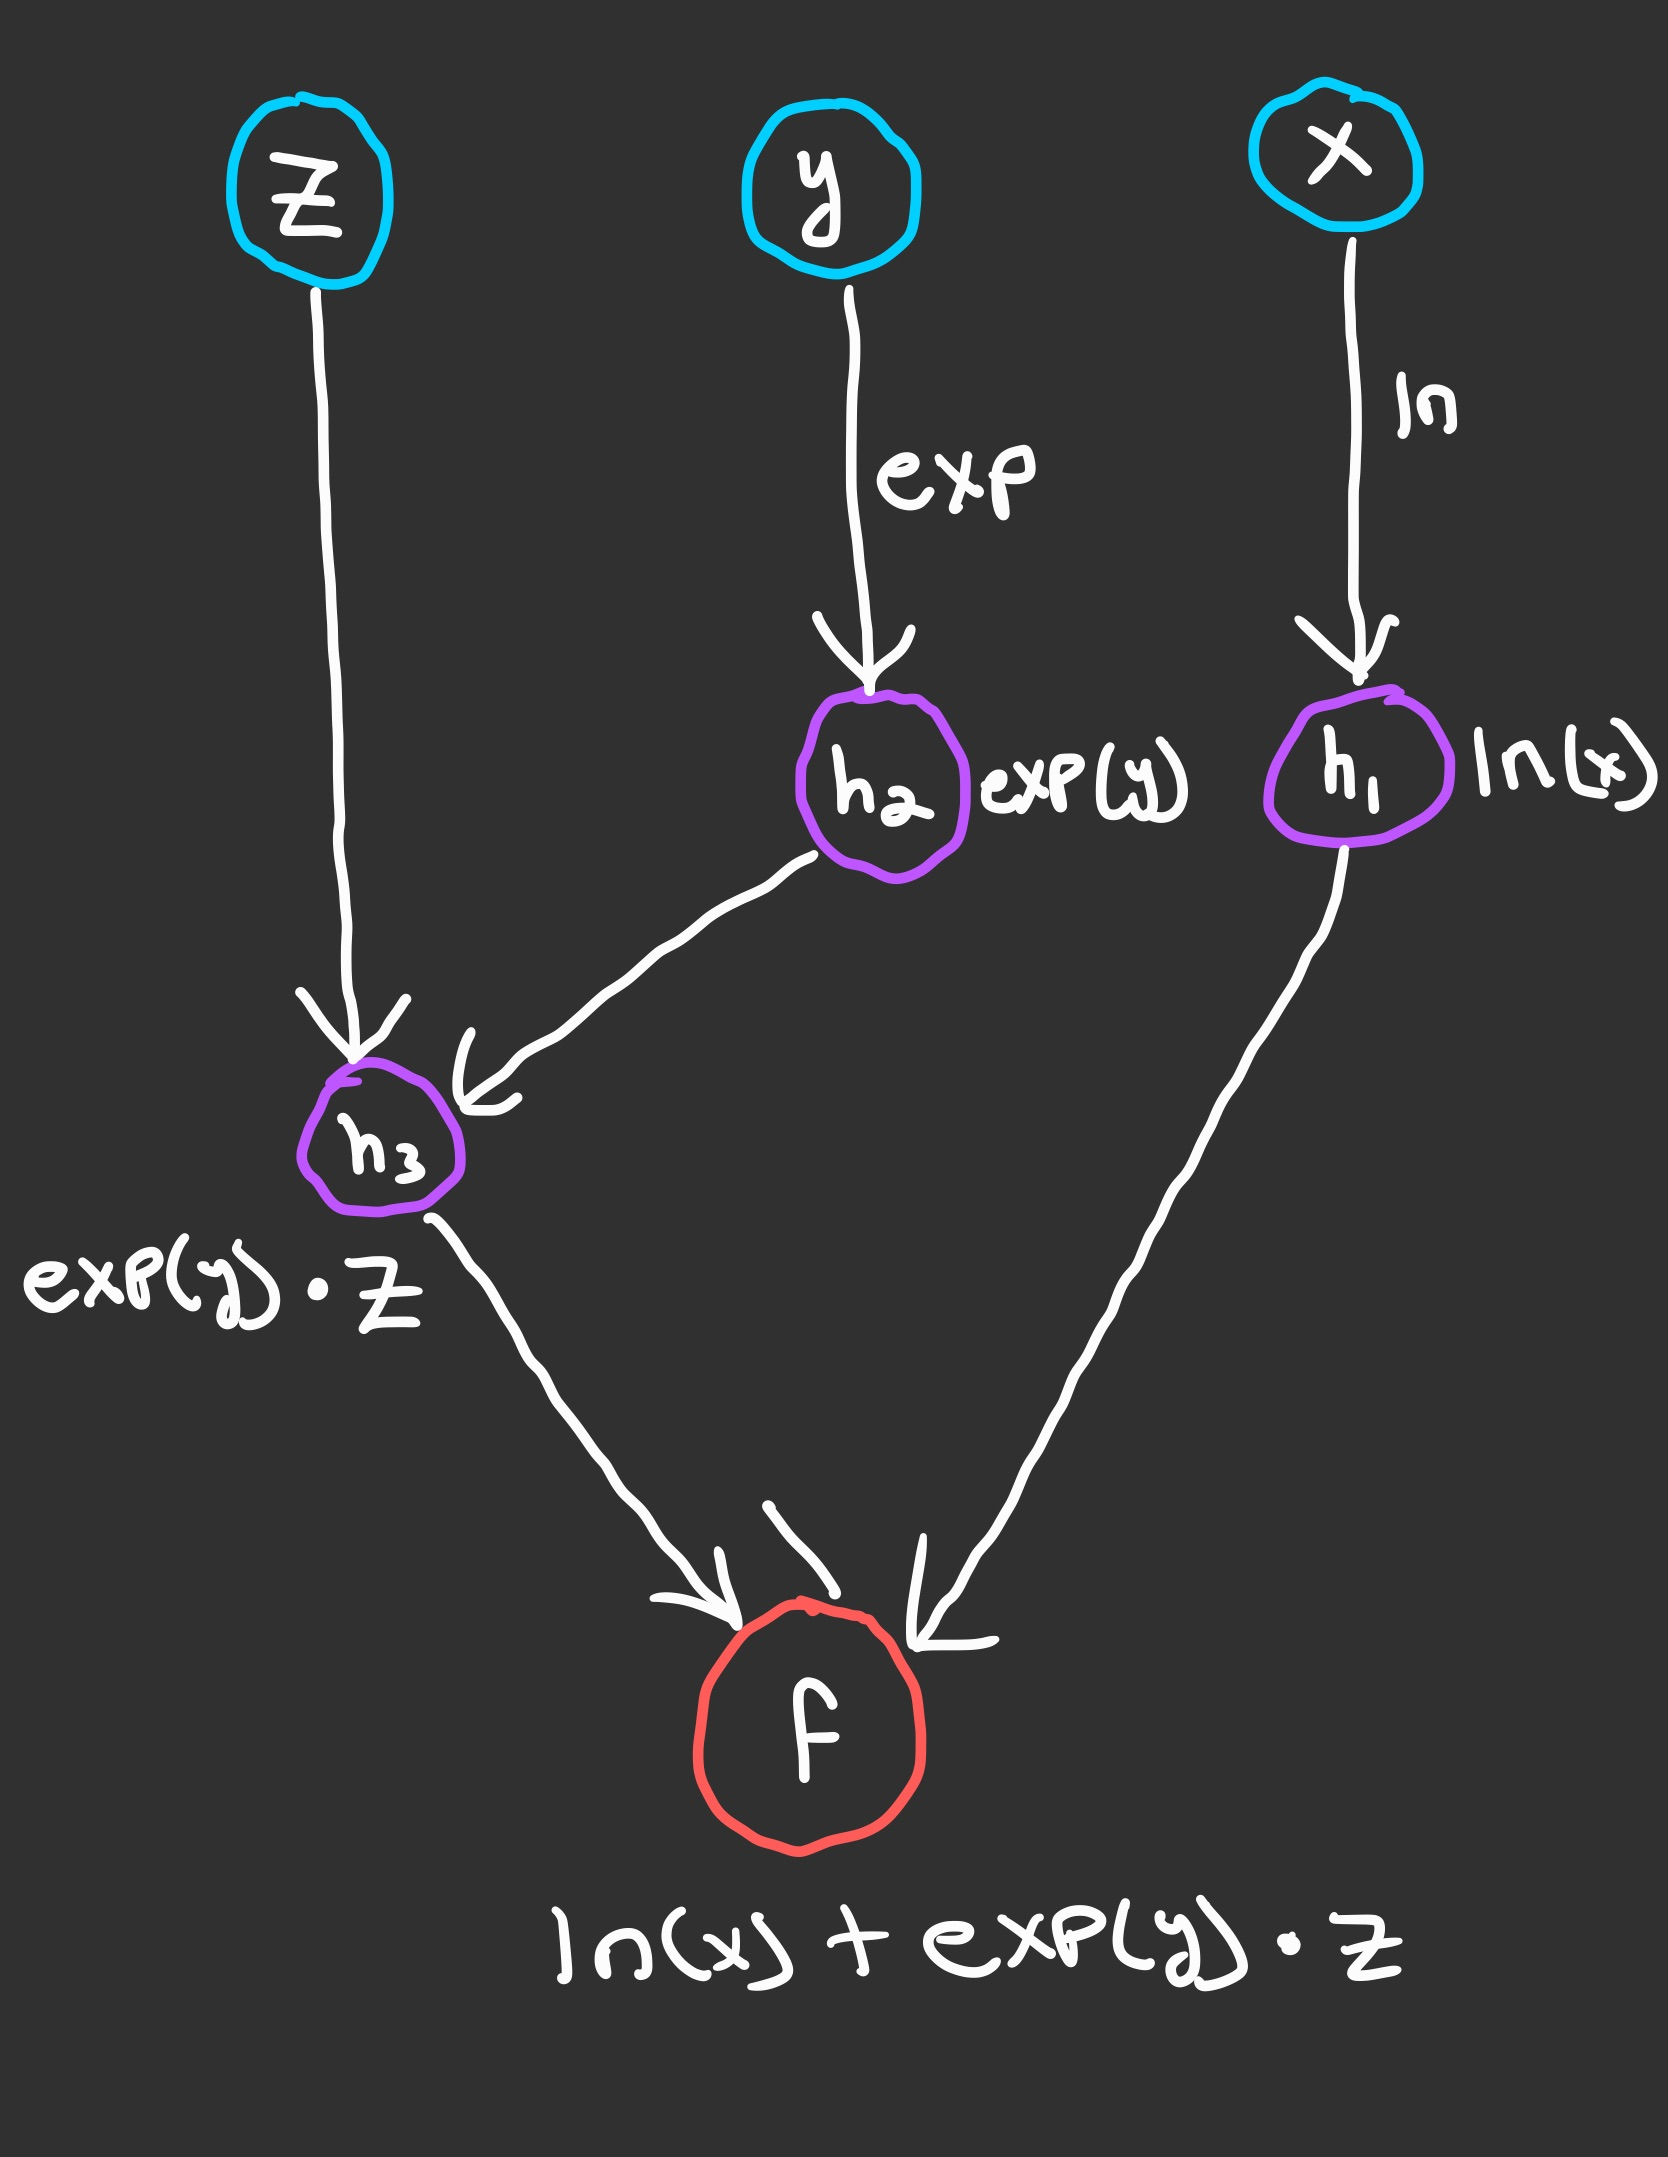
\includegraphics[width=0.6\textwidth]{figures/computation_graph.jpg}
        \end{figure}}
        \item Run the forward propagation and evaluate $f$ and $h_i$ ($i=1, 2, \dots$) at $[x, y, z] = [1, 3, 2]$.\\
        \solution{$h_1 = \ln x = \ln(1) = 0.0 \quad
        h_2 = \exp(y) = \exp(3) = 20.0855 \quad
        h_3 = h_2 \cdot z = 20.0855 \times 2 = 40.1711$ \\
        Final Output:
        $f = h_1 + h_3 = 0.0 + 40.1711 = 40.1711$}
        \item Run the backward propagation and give partial derivatives for each intermediate operation, i.e., $\frac{\partial h_i}{\partial x}$, $\frac{\partial h_j}{\partial h_i}$, and $\frac{\partial f}{\partial h_i}$. Evaluate the partial derivatives at $[x, y, z] = [1, 3, 2]$.\\
        \solution{
        $\frac{\partial f}{\partial h_1} = \frac{\partial}{\partial h_1} (h_1 + h_3) = 1,
        \frac{\partial f}{\partial h_3} = \frac{\partial}{\partial h_3} (h_1 + h_3) = 1,
        \frac{\partial h_3}{\partial h_2} = \frac{\partial}{\partial h_2} (h_2 \cdot z) = z = 2,
        \frac{\partial h_3}{\partial z} = \frac{\partial}{\partial z} (h_2 \cdot z) = h_2 = e^3 = 20.0855,
        \frac{\partial h_1}{\partial x} = \frac{\partial}{\partial x} (\ln x) = \frac{1}{x} = \frac{1}{1} = 1,
        \frac{\partial h_2}{\partial y} = \frac{\partial}{\partial y} (\exp(y)) = \exp(y) = e^3 = 20.0855.$ \\
        Since some variables do not directly depend on others, their partial derivatives are zero:
        $\frac{\partial h_1}{\partial y} = 0, \quad
        \frac{\partial h_1}{\partial z} = 0, \quad
        \frac{\partial h_2}{\partial x} = 0, \quad
        \frac{\partial h_2}{\partial z} = 0, \quad
        \frac{\partial h_3}{\partial x} = 0.$}
        \item Aggregate the results in (c) and evaluate the partial derivatives $\frac{\partial f}{\partial x}, \frac{\partial f}{\partial y}, \frac{\partial f}{\partial z}$ with chain rule. Show your work.\\
        \solution{
        $\frac{\partial f}{\partial x} = \frac{\partial f}{\partial h_1} \cdot \frac{\partial h_1}{\partial x}$ \\
        Substituting known values:
        $\frac{\partial f}{\partial x} = 1 \cdot \frac{1}{x} = 1 \cdot \frac{1}{1} = 1.0$ \\
        $\frac{\partial f}{\partial y} = \frac{\partial f}{\partial h_3} \cdot \frac{\partial h_3}{\partial h_2} \cdot \frac{\partial h_2}{\partial y}$ \\
        Substituting known values:
        $\frac{\partial f}{\partial y} = 1 \cdot 2 \cdot e^3 = 1 \cdot 2 \cdot 20.0855 = 40.1711$ \\
        $\frac{\partial f}{\partial z} = \frac{\partial f}{\partial h_3} \cdot \frac{\partial h_3}{\partial z}$ \\
        Substituting known values:
        $\frac{\partial f}{\partial z} = 1 \cdot e^3 = 1 \cdot 20.0855 = 20.0855$ \\
        Thus, the total derivatives evaluated at \( (x, y, z) = (1, 3, 2) \) are:
        $
        \frac{\partial f}{\partial x} = 1.0, \quad
        \frac{\partial f}{\partial y} = 40.1711, \quad
        \frac{\partial f}{\partial z} = 20.0855.
        $}
    \end{enumerate}



\clearpage
  

\section{Programming}
In this programming homework, we will
\begin{itemize}
    \item implement MLP-based classifiers for the sentiment classification task of homework 1.
\end{itemize}

\noindent \paragraph{Skeleton Code and Structure:}
The code base for this homework can be found at MyClasses Files under the \texttt{hw3} directory. Your task is to fill in the missing parts in the skeleton code, following the requirements, guidance, and tips provided in this pdf and the comments in the corresponding .py files.
The code base has the following structure:
\begin{itemize}
    \item \texttt{mlp.py} reuse the sentiment classifier on movie reviews you implemented in homework 1, with additional requirements to implement MLP-based classifier architectures and forward pass .
    \item \texttt{main.py} provides the entry point to run your implementations \texttt{mlp.py}
    \item \texttt{hw3.md} provides instructions on how to setup the environment and run each part of the homework in \texttt{main.py}
\end{itemize}

\noindent \todo{} ---
Your tasks include
1) generate plots and/or write short answers based on the results of running the code; 2) fill in the blanks in the skeleton to complete the code. We will explicitly mark these plotting, written answer, and filling-in-the-blank tasks as \todo{} in the following descriptions, as well as a \textcolor{blue}{\texttt{\textbf{\#~TODO}}} at the corresponding blank in the code. \\

\noindent \todo{} (Copy from your HW1). We are reusing most of the \texttt{model.py} from homework 1 as the starting point for the \texttt{mlp.py} - you will see in the skeleton that they look very similar. Moreover, in order to make the skeleton complete, for all the \textcolor{blue}{\texttt{\textbf{\#~TODO (Copy from your HW1)}}}, please fill in the blank below them by copying and pasting the corresponding implementations you wrote for homework 1 (i.e. the corresponding \textcolor{blue}{\texttt{\textbf{\#~TODO}}} in homework 1.)

\noindent \paragraph{Submission:} Your submission should contain two parts: 1) plots and short answers under the corresponding questions below; and 2) your completion of the skeleton code base, in a \texttt{.zip} file

\subsection{MLP-based Sentiment Classifier}
In both homework 1 \& 2, our implementation of the \texttt{SentimentClassifer} is essentially a single-layer feedforward neural network that maps input features directly to 2-dimensional output logits. In this part of the programming homework, we will expand the architecture of our classifier to multi-layer perceptron (MLP). 

\subsubsection{Reuse Your HW1 Implementation}
\todo{} (Copy from your HW1): for all the \textcolor{blue}{\texttt{\textbf{\#~TODO (Copy from your HW1)}}} in \texttt{mlp.py}, please fill in the blank below them by copying and pasting the corresponding implementations you wrote for homework 1 (i.e. the corresponding \textcolor{blue}{\texttt{\textbf{\#~TODO}}} in the \texttt{model.py} in homework 1).

\subsubsection{Build MLPs}
\label{subsubsec: build mlps}
Remember from the lecture that MLP is a multi-layer feedforward network with perceptrons as its nodes. A perceptron consists of non-linear activation of the affine (linear) transformation of inputs.
\\\\
\noindent \todo{}: Complete the \texttt{\_\_init\_\_} and \texttt{forward} function of the \texttt{SentimentClassifier} class in \texttt{mlp.py} to build MLP classifiers that supports custom specification of architecture (i.e. number and dimension of hidden layers)\\
\noindent \textbf{Hint}: check the comments in the code for specific requirements about input, output, and implementation. Also, check out the document of \href{https://pytorch.org/docs/stable/generated/torch.nn.ModuleList.html}{nn.ModuleList} about how to define and implement forward pass of MLPs as a stack of layers.

\subsubsection{Train and Evaluate MLPs}
We provide in \texttt{main.py} several MLP configurations and corresponding recipes for training them.\\\\
\noindent\todo{} Once you finished \autoref{subsubsec: build mlps}, you can run \texttt{load\_data\_mlp} and \texttt{explore\_mlp\_structures} to train and evaluate these MLPs and paste two sets of plots here:
\begin{itemize}
    \item 4 plots of train \& dev loss for each MLP configuration
    \item 2 plots of dev losses and accuracies across MLP configurations
\end{itemize}
and describe in 2-3 sentences your findings.\\
\noindent \textbf{Hint}: what are the trends of train \& dev loss and are they consistent across different configurations? Is deeper models always better? Why?\\
\noindent {\color{red}{your plots and answer:}}\\
% uncomment the following blocks to include your plots
\begin{figure}[h] 
    \centering
    \subfloat[No Hidden Layer]{
        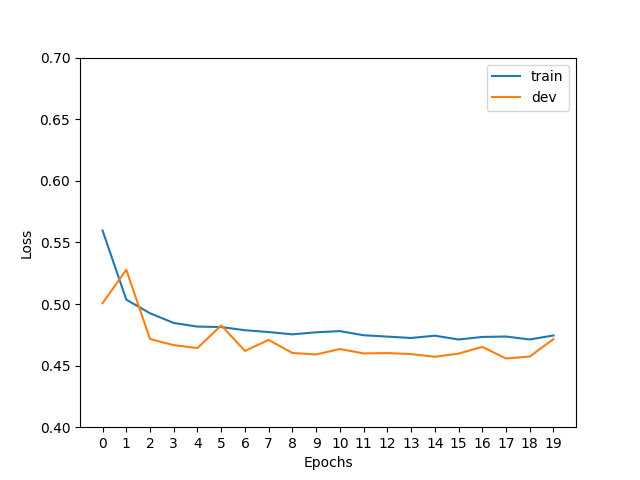
\includegraphics[width=0.23\textwidth]{figures/mlp_structure_None_loss.png}
        }
    \hfill
    \subfloat[1 Hidden Layer]{
        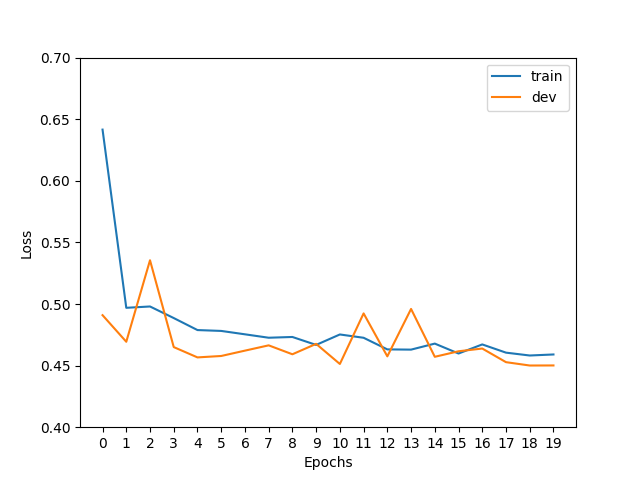
\includegraphics[width=0.23\textwidth]{figures/mlp_structure_512_loss.png}
        }
    \hfill
    \subfloat[2 Hidden Layers]{
        \includegraphics[width=0.23\textwidth]{figures/mlp_structure_512 - 512_loss.png}
        }
    \hfill
    \subfloat[3 Hidden Layers]{
        \includegraphics[width=0.23\textwidth]{figures/mlp_structure_512 - 512 - 512_loss.png}
        }
    \caption{loss of different MLP architectures}
\end{figure}
\begin{figure}[h] 
    \centering
    \subfloat[dev loss of different MLP architectures]{
        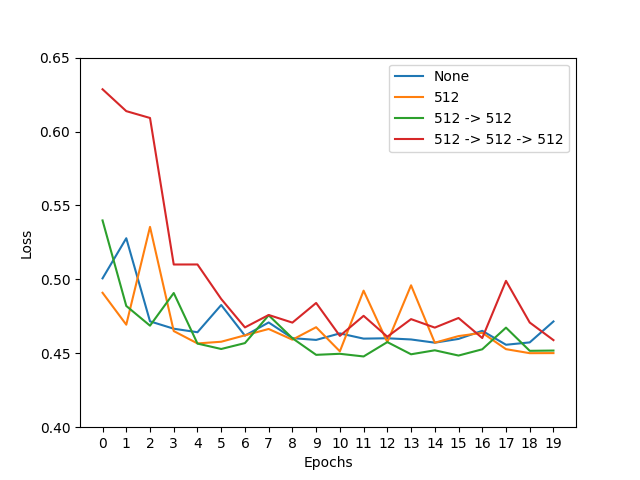
\includegraphics[width=0.45\textwidth]{figures/all_mlp_structures_loss.png}
        }
    \hfill
    \subfloat[dev acc of different MLP architectures]{
        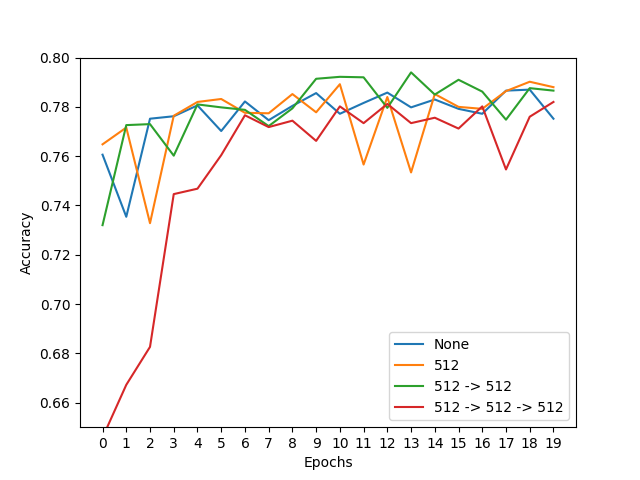
\includegraphics[width=0.45\textwidth]{figures/all_mlp_structures_acc.png}
        }
    \caption{loss and acc of different MLP architectures}
\end{figure}    
\solution{ \\ From the provided loss and accuracy plots, we observe that deeper MLP models (with more hidden layers) do not always lead to better performance. The training and development (dev) loss decrease over epochs for all architectures, but the rate of improvement varies. The simplest model (None) and the 512->512 model generally perform better in terms of stability, while the deeper 512->512->512 model initially struggles but catches up later. However, the deepest model tends to have more fluctuations and does not consistently outperform shallower architectures, likely due to increased complexity leading to optimization challenges or overfitting.}

\subsubsection{Embrace Non-linearity: The Activation Functions}
Remember we have learned why adding non-linearity is useful in neural nets and gotten familiar with several non-linear activation functions both in the class and \autoref{sec: activation}. Now it is time to try them out in our MLPs! \\
\textbf{Note: for the following TODO and the TODO in \autoref{subsubsec: lr}, we fix the MLP structure to be with a single 512-dimension hidden layer, as specified in the code. You only need to run experiments on this architecture}.\\\\
\noindent\todo{}: Read and complete the missing lines of the two following functions:
\begin{itemize}
    \item \texttt{\_\_init\_\_} function of the \texttt{SentimentClassifier} class: define different activation functions given the input \texttt{activation} type.\\
    \textbf{Hint}: we have provided you with a demonstration of defining the Sigmoid activation, you can search for the other \texttt{nn.<activation>} in PyTorch documentation.\\
    \item \texttt{explore\_mlp\_activations} in \texttt{main.py}: iterate over the activation options, define the corresponding training configurations, train and evaluate the model, and visualize the results. Note: you only need to generate the plots of dev loss and dev acc across different configurations, by calling \texttt{visualize\_configs}, you \textbf{do not} need to plot the train-dev loss curves for each configuration (i.e. no need to call \texttt{visualize\_epochs}). We provide you with a few choices of common activation functions, but feel free to try out the others.\\
    \textbf{Hint}: You can refer to \texttt{explore\_mlp\_structure} as a demonstration of how to define training configurations with fixed hyper-parameters \& iterate over hyper-parameters/design choices of interests (e.g. hidden dimensions, choice of activation), and plot the evaluation results across configurations. 
\end{itemize}
Once you complete the above functions, run \texttt{explore\_mlp\_activations} and paste the two generated plots here. Describe in 2-3 sentences your findings.\\
\noindent {\color{red}{your plots and answer:}}\\
% uncomment the following blocks to include your plots
\begin{figure}[h] 
    \centering
    \subfloat[dev loss of different activations]{
        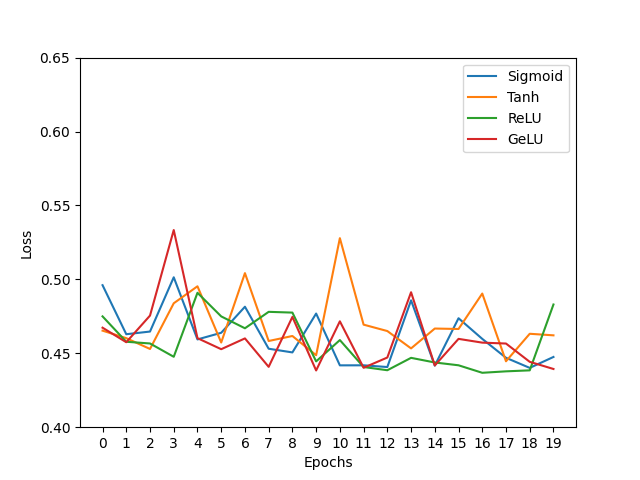
\includegraphics[width=0.45\textwidth]{figures/all_mlp_activations_loss.png}
        }
    \hfill
    \subfloat[dev acc of different MLP architectures]{
        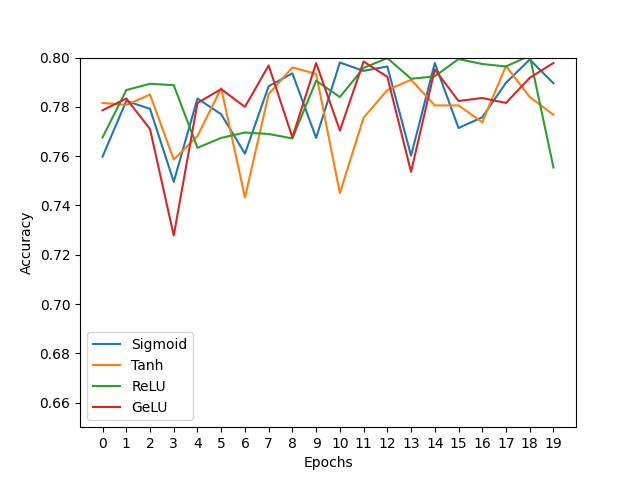
\includegraphics[width=0.45\textwidth]{figures/all_mlp_activations_acc.png}
        }
    \caption{loss and acc of different activations}
\end{figure}\\
\solution{ \\ The plots of dev accuracy and dev loss across different activation functions show variations in how well each activation enables learning and generalization, which is relatively similar for each function. Some activations seem to result in faster convergence and lower loss (such as ReLU), while others, struggle at times and experience spikes of loss / low accuracies (such as GeLU). Overall, the choice of activation function significantly influences both accuracy and loss trends, highlighting the importance of selecting an appropriate function for MLP architectures.}

\subsubsection{Hyper-parameter Tuning: Learning Rate}
\label{subsubsec: lr}
The training process mostly involves learning model parameters, which are automatically performed by gradient-based methods. However, certain parameters are ``unlearnable" through gradient optimization while playing a crucial role in affecting model performance, for example, learning rate and batch size. We typically refer to these parameters as \textit{Hyper-parameters}.

We will now take the first step to tune these hyper-parameters by exploring the choices of one of the most important one - learning rate, on our MLP. (There are lots of tutorials on how to tune the learning rate manually or automatically in practice, for example \href{https://www.kaggle.com/code/residentmario/tuning-your-learning-rate}{this note} can serve as a starting point.)\\\\
\noindent\todo{}: Read and complete the missing lines in \texttt{explore\_mlp\_learning\_rates} in \texttt{main.py} to iterate over different learning rate values, define the training configurations, train and evaluate the model, and visualize the results. Note: same as above, you only need to generate the plots of dev loss and dev acc across different configurations, by calling \texttt{visualize\_configs}, you \textbf{do not} need to plot the train-dev loss curves for each configuration (i.e. no need to call \texttt{visualize\_epochs}). We provide you with the default learning rate we set to start with, and we encourage you to add more learning rate values to explore and include in your final plots curves of \textbf{at least 4 different representative learning rates.}\\
\noindent\textbf{Hint}: again, you can checkout \texttt{explore\_mlp\_structure} as a demonstration for how to perform hyper-parameter search.\\
Once you complete the above functions, run \texttt{explore\_mlp\_learning\_rates} and paste the two generated plots here. Describe in 2-3 sentences your findings.\\
\noindent {\color{red}{your plots and answer:}}\\
% uncomment the following blocks to include your plots
\begin{figure}[h] 
    \centering
    \subfloat[dev loss of different learning rates]{
        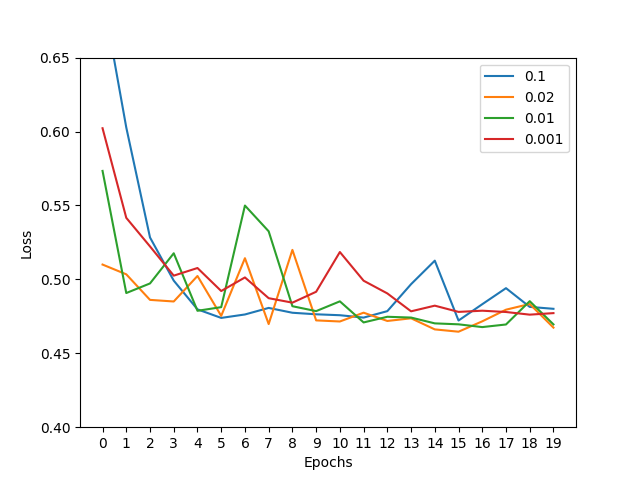
\includegraphics[width=0.45\textwidth]{figures/all_mlp_lrs_loss.png}
        }
    \hfill
    \subfloat[dev acc of different MLP architectures]{
        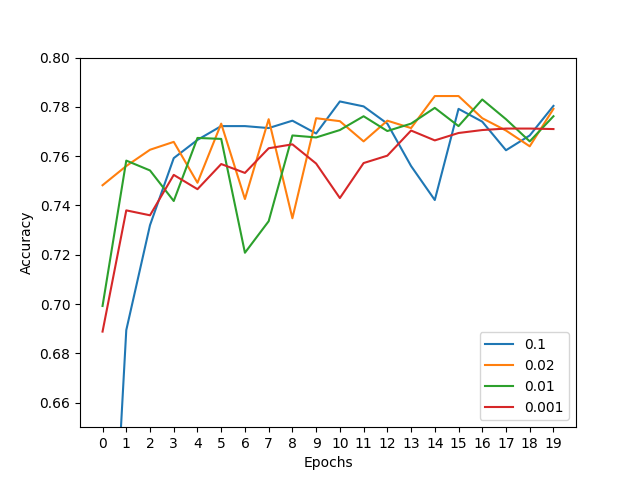
\includegraphics[width=0.45\textwidth]{figures/all_mlp_lrs_acc.png}
        }
    \caption{loss and acc of different learning rates}
\end{figure}\\

\bibliographystyle{apalike}
\bibliography{ref}
\noindent\solution{ \\ From the accuracy plot, we see that learning rates of 0.02 and 0.01 provide the most stable and highest accuracy, while 0.1 starts slower but catches up later. The loss plot shows that 0.1 initially has a high loss but converges quickly, whereas 0.001 decreases steadily but at a slower rate, potentially struggling to escape local minima. Overall, learning rates of 0.02 and 0.01 strike a good balance between stability and convergence speed, although the learning rate of 0.001 became very stable after Epoch 13 with a slightly lower ending accuracy.}
\end{document}

\bibliographystyle{apalike}
\bibliography{ref}

\end{document}